\fancyhead[C]{Section 16.5}
\fancyhead[R]{\daytwentyfive}

\section*{\centering Chapter 16.5: Parametric Surfaces}

{\small \textbf{G5: Parameterization.} I can find parametric equations for common curves, such as line segments, graphs of functions of one variable, circles, and ellipses.  I can match given parametric equations to Cartesian equations and graphs. I can parameterize common surfaces, such as planes, quadric surfaces, and functions of two variables.

\textbf{V4: Surface Integrals.} I can set up and compute surface integrals for scalar and vector valued functions.}

\subsection*{Mechanics}
\begin{enumerate}
	\item \question{Consider the surface cut from the parabolic cylinder $y=4-x^2$ by the planes $z=0$, $z=2$, and $y=0$. Sketch $S$ and find a parameterization of $S$.}{% answer here
        
        }
        {% solution here
        
        }
    \item \question{Consider the surface given by $x^2+y^2+z^2=4$, where  $z\geq \sqrt{3}$. Sketch $S$, parametrize $S$ and find the surface area of $S$. }{% answer here
        
        }
        {% solution here
        
        } 
	\item \question{Find the area of the surface cut from the ``nose" of the paraboloid $x=1-y^2-z^2$ by the $yz$-plane.}{% answer here
        
        }
        {% solution here
        
        } 
    \item \question{Find the area of the part of the surface $z=xy$ that lies within the cylinder $x^2+y^2=1$. }{% answer here
        
        }
        {% solution here
        
        } 
\end{enumerate}
\subsection*{Applications}
\begin{enumerate}[resume]
    \item \question{Recall from Calculus class that one can form a surface by revolving the graph of a \emph{non-negative} function $y=f(x)$ about the $x$-axis. Translating this into the language of parameterized surfaces, convince yourself that a parameterization can be given by 
    \begin{equation*}
        r(x,\theta) = (x,f(x)\cos \theta, f(x)\sin \theta)
    \end{equation*}
    \emph{[Hint: Each $x$-cross section is a circle with what radius?]} A typical (American) football can be roughly modeled as the revolution of the area of intersection of the two circles $x^2+(y-1)^2=4$ and $x^2+(y+1)^2 =4$ about the $x$-axis. Set up a surface integral to compute the surface area of a football. [Warning: this is not to scale!!]

    \begin{multicols}{2}
    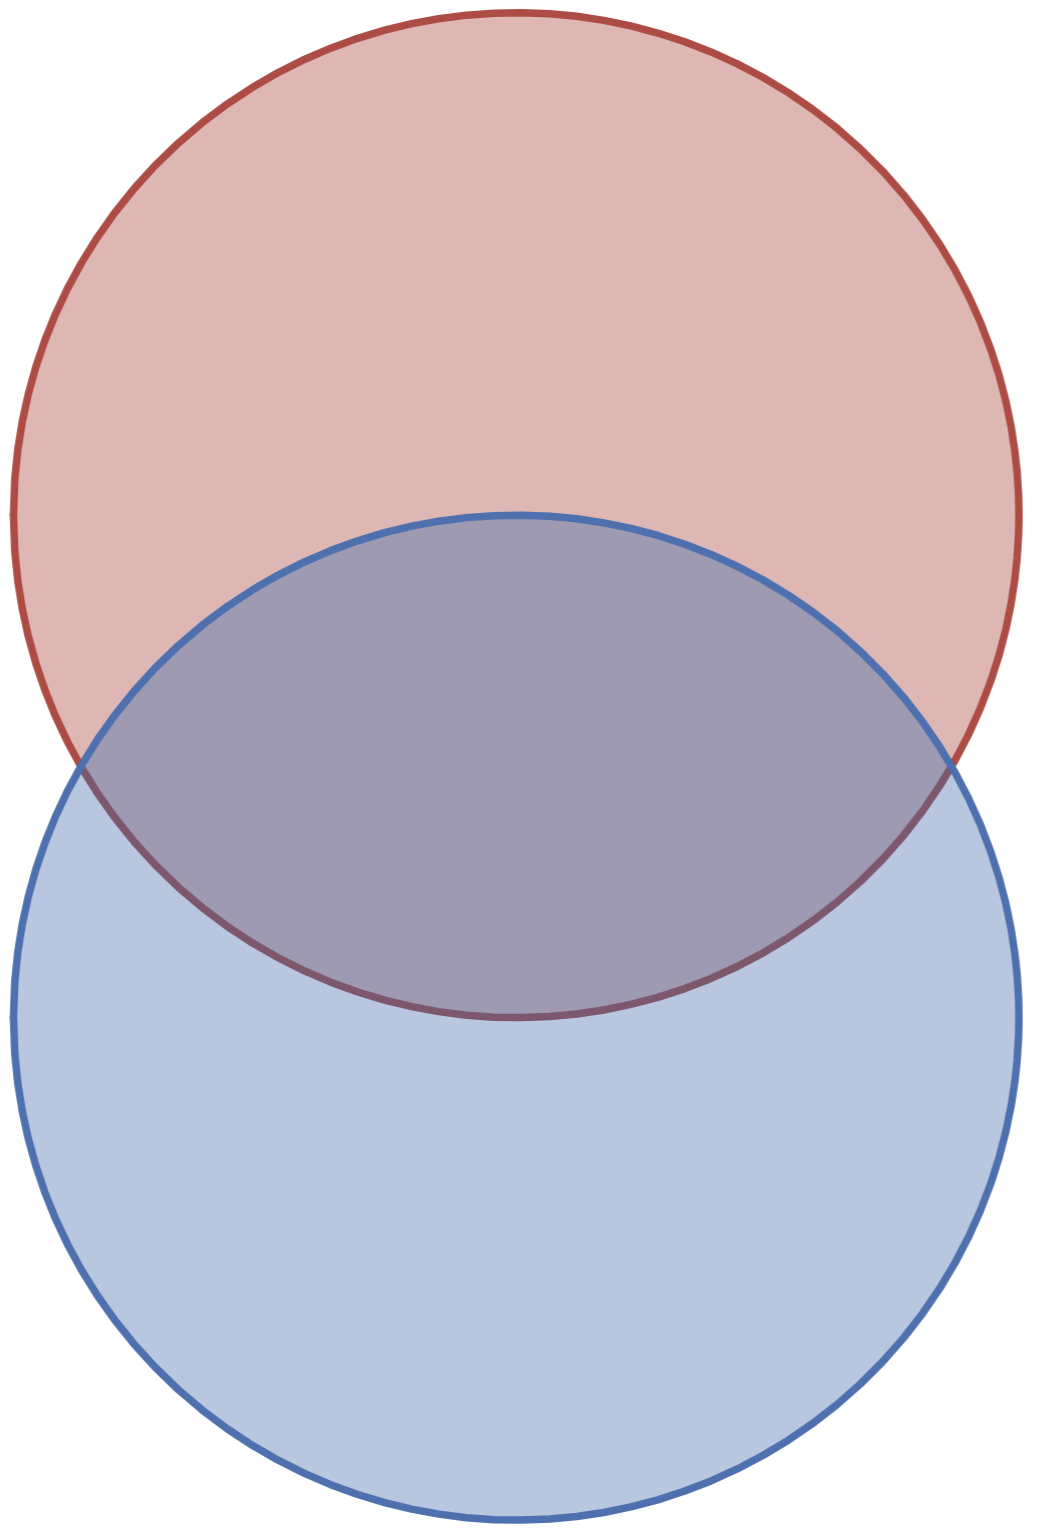
\includegraphics[width=.22\textwidth,alt={two intersecting disks}]{model football.png}

    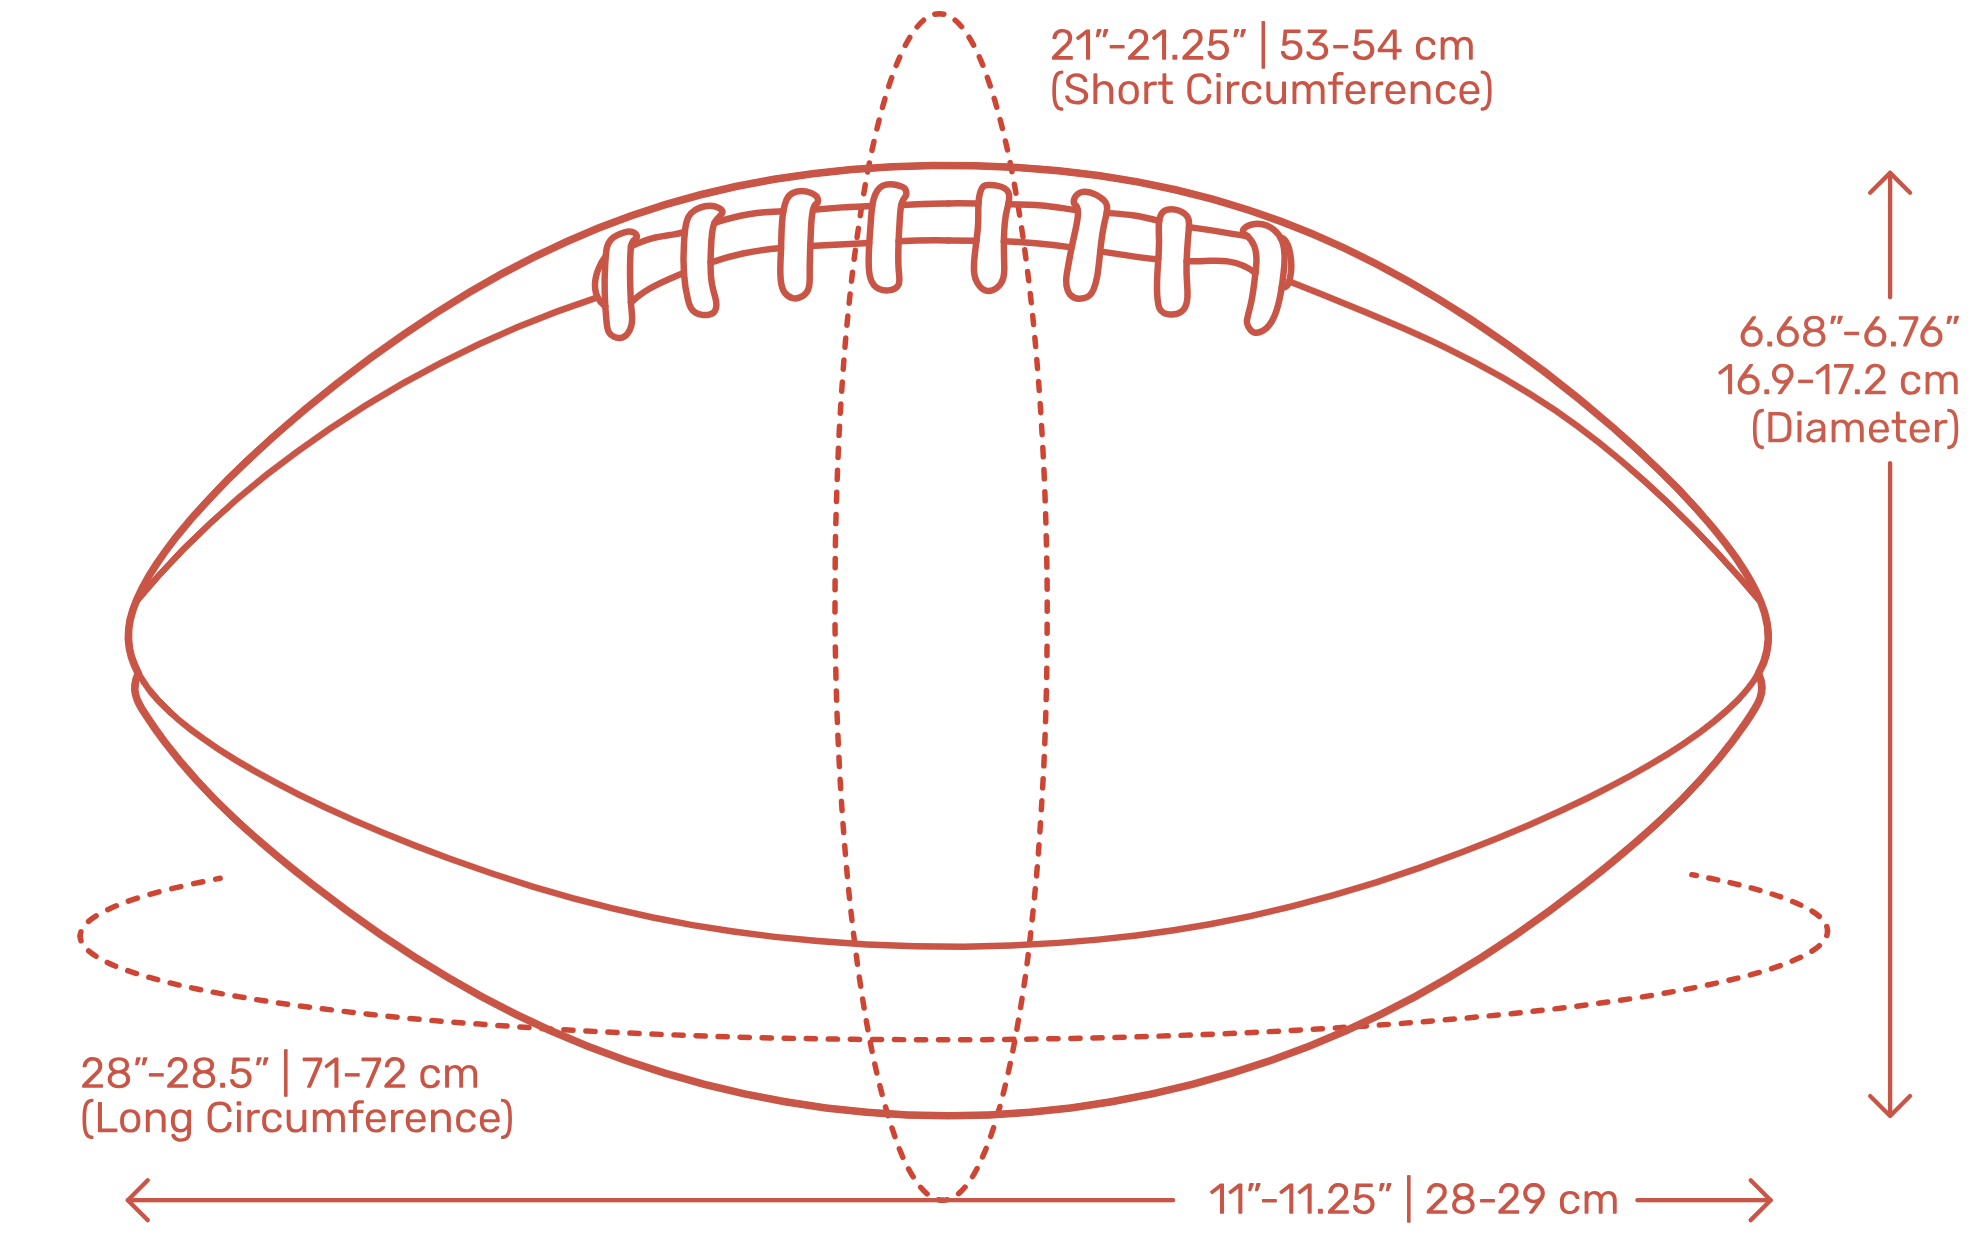
\includegraphics[width=.45\textwidth,alt={american football}]{real football.png}
    \end{multicols}
    }{% answer here
        
        }
        {% solution here
        
        } 
\end{enumerate}

\pagebreak 

\subsection*{Extensions}
\begin{enumerate}[resume]

	\item \question{The tangent plane at a point $P_0=(f(u_0,v_0),g(u_0,v_0),h(u_0,v_0))$ on a parameterized surface $\br(u,v)=\langle f(u,v), g(u,v) ,h(u,v)\rangle$ is the plane through $P_0$ with normal vector equal to $\br_u (u_0,v_0)\times\br_v(u_0,v_0)$.
	
	Use this to find an equation to the tangent plane of the surface parameterized by $\br(r,\theta)=(r\cos(\theta))\bi+(r\sin(\theta))\bj+r\bk$, with $r\geq 0, 0\leq\theta\leq 2\pi$ at the point where $(r,\theta)=(2,\pi/4)$.
	
	What is a Cartesian equation for this surface?  Sketch it and the tangent plane.}{% answer here
        
        }
        {% solution here
        
        }
    \item \question{The notion of curvature for curves that we explored in Chapter 13.4 has an extension for parametric surfaces, and is fundamental in a field of math called \emph{differential geometry}. Recall from the above problem that the \emph{unit} normal vector to a parameterized surface $\br(u,v)$ is given by the vector $\bn = \frac{\br_u\times \br_v}{\|\br_u\times \br_v\|}$. Consider the following scalar quantities for the surface $\br(u,v)$:
    \begin{align*}
        E &= \br_u \cdot \br_u\\
        F &= \br_u\cdot \br_v\\
        G &= \br_v\cdot \br_v\\
        L &= \br_{uu}\cdot \bn\\
        M &= \br_{uv}\cdot \bn\\
        N &= \br_{vv}\cdot \bn
    \end{align*}
    The \emph{Gaussian curvature} of the surface is given by the quantity
    \begin{equation*}
        \kappa = \frac{LN-M^2}{EG-F^2}
    \end{equation*}
    Verify that the Gaussian curvature at any point on a sphere of radius $r$ is $\frac{1}{r^2}$. Does this result remind you of how the curvature of certain curves are also constant?}{% answer here
        
        }
        {% solution here
        
        }
\end{enumerate}

\iftoggle{answers}{
\begin{center}{\large \textbf{Math 2551 Worksheet Answers: Surfaces}}
\end{center}

\begin{enumerate}
	
	\item One answer: $\br(u,v)=\langle u, 4-u^2, v\rangle$, $-2\leq u\leq 2, 0\leq v\leq 2$. 
	
	\item One answer: $\br(\phi,\theta)=\langle 2\sin(\phi)\cos(\theta), 2\sin(\phi)\sin(\theta),2\cos(\phi)\rangle$ with $0\leq \phi \leq \pi/6$ and $0\leq \theta \leq 2\pi$.\\
	SA: $8\pi \left(1-\frac{\sqrt{3}}{2} \right)$
	
	\item The tangent plane is $-\sqrt{2}(x-\sqrt{2})-\sqrt{2}(y-\sqrt{2})+2(z-2)=0$. This is the cone $z=\sqrt{x^2+y^2}$.
	
	\item $\dfrac{2}{3}\pi(2^{3/2}-1)$ 
	
	\item $\dfrac{\pi}{6}(5^{3/2}-1)$
\end{enumerate}

}{}
\iftoggle{solutions}
{
Solutions go here in the same format.
}{}